\chapter{Fundamentals of Plasma Physics}
\label{ch:fundamentals}

Quantifying the ion energy flux across a plasma sheath rests on a small set of foundational concepts: quasi-neutrality, Debye screening, the characteristic frequencies separating collective plasma behaviour from ordinary gas dynamics, the statistical description of particle velocities through distribution functions, and the collisional processes governing how closely a real plasma approaches the idealized kinetic picture. This chapter derives or motivates these building blocks from first principles -- the Debye length, the plasma and cyclotron frequencies, the Bohm velocity $u_{\mathrm{B}}$, and the moments of the ion distribution function $f_{\mathrm{i}}(v)$ that define the ion energy flux $\Gamma_{E}$ -- so later chapters can proceed without interruption.

\section{States of Matter, Ionization, and the Definition of a Plasma}
\label{sec:states-ionization}

\subsection{From Neutral Gas to Ionized Gas}

Matter is conventionally classified into four states -- solid, liquid, gas, and plasma -- ordered by increasing thermal energy per particle relative to the binding energy holding the constituents together. In a solid, particles occupy fixed lattice sites; melting frees translational motion; further heating produces a gas of freely streaming particles dominated by short binary collisions. Heated further, or supplied with sufficient energy through an applied field, irradiation, or shock compression, a fraction of the gas ionizes: an outer electron escapes its parent nucleus, producing a free electron and a positive ion. Once the ionized fraction is large enough that long-range Coulomb interactions dominate the medium's collective response, it is termed a \emph{plasma}, sometimes called the fourth state of matter.

Ionization alone does not make a plasma: a gas with a small free-charge population is, strictly, ionized, but unless those charges are numerous and mobile enough to screen electric fields collectively, the medium behaves as an ordinary, weakly conducting neutral gas. The formal criteria separating a plasma from a merely ionized gas -- many particles within a screening volume, a screening length much smaller than the system size, and collective response dominating over collisions with neutrals -- are developed quantitatively in Section~\ref{sec:frequencies}.

\subsection{Definition of a Plasma}

A plasma is a quasi-neutral gas of charged and neutral particles exhibiting \emph{collective behaviour}: the long-range Coulomb force means a charged particle's motion is influenced not merely by its nearest neighbours, as in an ordinary gas, but by the aggregate field of all other nearby charges. This lets a plasma support charge-density waves, screen imposed electrostatic perturbations over a finite distance, and -- of direct relevance here -- form thin, non-neutral boundary layers, the \emph{sheaths}, wherever it contacts a material surface. The plasma-sheath transition, and the associated Bohm criterion governing ion flow into the sheath, remains an actively debated topic \cite{ref0001,ref0015}.

Three ingredients recur in essentially every rigorous definition of a plasma: approximate charge neutrality on macroscopic scales, a screening length -- the Debye length -- much smaller than the system's dimensions, and a sufficiently large number of particles within a Debye-length sphere for a smoothly averaged electric field to be meaningful. These are examined in turn below.

\subsection{Ionization Energy and Partial Ionization}

The energy required to remove the first electron from a neutral atom or molecule, its first ionization energy $\chi_{\mathrm{ion}}$, sets the energy scale below which a gas remains almost entirely neutral. Representative values span roughly \SI{13.6}{\electronvolt} for atomic hydrogen and \SI{15.8}{\electronvolt} for argon, down to a few electronvolts for easily ionized alkali vapours such as caesium. Because a Maxwellian electron population (Section~\ref{sec:distributions}) has an exponentially small fraction of particles above $\chi_{\mathrm{ion}}$ whenever $k_{\mathrm{B}} T_{\mathrm{e}} \ll \chi_{\mathrm{ion}}$, most laboratory discharges operate with electron temperatures of only a few electronvolts even though the working gas's ionization energy is an order of magnitude larger; ionization is sustained by the high-energy tail of the electron distribution, so the steady-state degree of ionization $\alpha$ (Section~\ref{sec:collisions}) is exquisitely sensitive to that tail's shape, motivating non-Maxwellian-capable diagnostics of the electron distribution function \cite{ref0194,ref0213}.

\section{Quasi-Neutrality, Collective Behaviour, and Debye Shielding}
\label{ch02-sec:debye}

\subsection{Quasi-Neutrality}

On length scales large compared with a certain characteristic distance, a plasma is electrically neutral to a very high degree of approximation: the electron density $n_{\mathrm{e}}$ and the (possibly summed) ion density $n_{\mathrm{i}}$ satisfy
\begin{equation}
n_{\mathrm{e}} \approx Z n_{\mathrm{i}},
\label{eq:quasineutrality}
\end{equation}
even though the plasma is filled with free charges capable of sustaining large local fields. This apparent paradox is resolved because any small charge imbalance builds up a restoring field so strong that only a minute fractional imbalance, of order $(\lambda_{\mathrm{D}}/L)^{2}$ for a system of size $L$ and Debye length $\lambda_{\mathrm{D}}$, can be sustained in equilibrium: quasi-neutrality follows from the same screening physics that defines $\lambda_{\mathrm{D}}$, derived below. It is precisely because quasi-neutrality holds only outside thin boundary layers -- where it is deliberately violated -- that the plasma sheath exists as a distinguishable, non-neutral region whose thickness scales with $\lambda_{\mathrm{D}}$ \cite{ref0013,ref0023}.

\subsection{Collective Behaviour}

The distinguishing feature of a plasma, relative to a neutral gas, is that the dominant interactions among its particles are long-range and collective rather than short-range and binary: a neutral molecule interacts appreciably only with the few neighbours it collides with, whereas in a plasma the cooperative response of surrounding charges truncates the bare Coulomb interaction at a finite distance $\lambda_{\mathrm{D}}$ while a large number of particles, of order the plasma parameter $N_{\mathrm{D}} = n_{\mathrm{e}}\lambda_{\mathrm{D}}^{3}$, participate at once. This many-body character is what "collective behaviour" means, and it permits a plasma to support organized charge-density oscillations (Section~\ref{sec:frequencies}) and to generate self-consistent internal fields, such as the ambipolar presheath field, that regulate ion flow toward a bounding wall \cite{ref0006}.

\subsection{Derivation of the Debye Length}

Consider an infinite, uniform, quasi-neutral plasma with equilibrium density $n_{0}$, into which a small perturbing potential $\phi$ is introduced at the origin. The electrons, far more mobile than the ions, respond quickly and adopt a Boltzmann equilibrium along the perturbed potential,
\begin{equation}
n_{\mathrm{e}}(\mathbf{r}) = n_{0}\exp\!\left(\frac{e\phi(\mathbf{r})}{k_{\mathrm{B}} T_{\mathrm{e}}}\right),
\label{ch02-eq:electron-boltzmann}
\end{equation}
where $T_{\mathrm{e}}$ is the electron temperature (in energy units through $k_{\mathrm{B}}$), $e$ the elementary charge, and $\phi$ is measured relative to the unperturbed plasma potential. On the time scale over which electrons equilibrate, the heavier ions may be treated as an immobile uniform background of density $n_{0}$. Poisson's equation for the self-consistent potential then reads
\begin{equation}
\nabla^{2}\phi = -\frac{e}{\varepsilon_{0}}\left(n_{\mathrm{i}} - n_{\mathrm{e}}\right) = -\frac{e}{\varepsilon_{0}}\left[n_{0} - n_{0}\exp\!\left(\frac{e\phi}{k_{\mathrm{B}} T_{\mathrm{e}}}\right)\right].
\label{ch02-eq:poisson-full}
\end{equation}
For a small perturbation, $|e\phi| \ll k_{\mathrm{B}} T_{\mathrm{e}}$, linearizing the exponential reduces Equation~\eqref{ch02-eq:poisson-full} to
\begin{equation}
\nabla^{2}\phi = \frac{n_{0} e^{2}}{\varepsilon_{0} k_{\mathrm{B}} T_{\mathrm{e}}}\,\phi \equiv \frac{\phi}{\lambda_{\mathrm{D}}^{2}},
\label{eq:poisson-linear}
\end{equation}
which defines the electron Debye length
\begin{equation}
\lambda_{\mathrm{D}} \equiv \left(\frac{\varepsilon_{0} k_{\mathrm{B}} T_{\mathrm{e}}}{n_{0} e^{2}}\right)^{1/2}.
\label{ch02-eq:debye-length}
\end{equation}
For a spherically symmetric point-charge perturbation of magnitude $q$, the solution of Equation~\eqref{eq:poisson-linear} vanishing at infinity is the Yukawa, or screened Coulomb, form
\begin{equation}
\phi(r) = \frac{q}{4\pi\varepsilon_{0} r}\exp\!\left(-\frac{r}{\lambda_{\mathrm{D}}}\right).
\label{eq:screened-potential}
\end{equation}
The bare Coulomb potential $q/4\pi\varepsilon_{0} r$ is thus exponentially attenuated beyond a distance of order $\lambda_{\mathrm{D}}$: collective rearrangement of the electrons confines the influence of any single charge, or an imposed boundary potential such as a wall's, to a shell of thickness $\sim \lambda_{\mathrm{D}}$ (Figure~\ref{fig:debye-shielding}). When both species respond self-consistently -- electrons via Equation~\eqref{ch02-eq:electron-boltzmann} and ions via an analogous factor at temperature $T_{\mathrm{i}}$ -- the linearized analysis yields the total Debye length
\begin{equation}
\frac{1}{\lambda_{\mathrm{D}}^{2}} = \frac{n_{0} e^{2}}{\varepsilon_{0}}\left(\frac{1}{k_{\mathrm{B}} T_{\mathrm{e}}} + \frac{1}{k_{\mathrm{B}} T_{\mathrm{i}}}\right),
\label{eq:debye-total}
\end{equation}
which reduces to Equation~\eqref{ch02-eq:debye-length} for $T_{\mathrm{e}} \gg T_{\mathrm{i}}$, but must be retained in full where the ions are not cold, as in the presheath, where they have already been accelerated.

\begin{figure}[htbp]
\centering
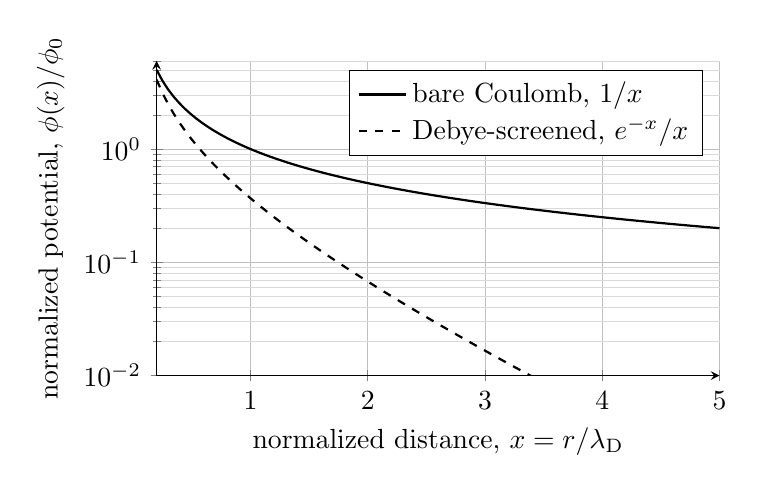
\begin{tikzpicture}
\begin{axis}[
 width=0.72\linewidth,
 height=0.46\linewidth,
 xlabel={normalized distance, $x = r/\lambda_{\mathrm{D}}$},
 ylabel={normalized potential, $\phi(x)/\phi_{0}$},
 ymode=log,
 xmin=0.2, xmax=5,
 ymin=0.01, ymax=6,
 grid=both,
 grid style={line width=0.1pt, draw=gray!30},
 major grid style={line width=0.2pt, draw=gray!50},
 legend pos=north east,
 legend cell align={left},
 axis lines=left,
]
\addplot[black, thick, domain=0.2:5, samples=100] {1/x};
\addlegendentry{bare Coulomb, $1/x$}
\addplot[black, thick, dashed, domain=0.2:5, samples=100] {exp(-x)/x};
\addlegendentry{Debye-screened, $e^{-x}/x$}
\end{axis}
\end{tikzpicture}
\caption{Schematic comparison of the bare-Coulomb potential $1/x$ and the Debye-screened potential $e^{-x}/x$, from Equation~\eqref{eq:screened-potential} in normalized units $x = r/\lambda_{\mathrm{D}}$. The curves are generated from the closed-form expressions only and do not represent measured or simulated data.}
\label{fig:debye-shielding}
\end{figure}

\subsection{The Debye Sphere and the Plasma Parameter}

The Debye length is a genuine screening scale only if enough particles lie within a sphere of radius $\lambda_{\mathrm{D}}$ for the mean-field treatment of Equation~\eqref{ch02-eq:electron-boltzmann} to hold; with only a handful of electrons in this volume, the screened potential would be dominated by discrete fluctuations rather than a smooth collective response. The number of electrons in a Debye sphere,
\begin{equation}
N_{\mathrm{D}} = \frac{4}{3}\pi \lambda_{\mathrm{D}}^{3} n_{\mathrm{e}},
\label{eq:debye-number}
\end{equation}
is the plasma parameter. A plasma in the sense used here is \emph{weakly coupled}, $N_{\mathrm{D}} \gg 1$, so the mean-field description is appropriate. Essentially all sheath, presheath, and ion energy flux theory developed later implicitly assumes this regime, characteristic of laboratory gas discharges and space plasmas.

\section{Characteristic Frequencies and the Formal Criteria for a Plasma}
\label{sec:frequencies}

\subsection{The Electron Plasma Frequency}

Debye shielding describes the static, equilibrium response of a plasma to a fixed perturbation. Its dynamical analogue is the plasma oscillation, whose frequency follows from a simple slab model. Consider a uniform, unmagnetized plasma in which a thin slab of electrons, initially coincident with a corresponding slab of (immobile) ions, is displaced by a small distance $\delta x$ in one dimension. The resulting charge separation produces, by Gauss's law, a uniform restoring field
\begin{equation}
E = \frac{n_{0} e\, \delta x}{\varepsilon_{0}}.
\label{eq:slab-field}
\end{equation}
The equation of motion for an electron of mass $m_{\mathrm{e}}$ in this field is
\begin{equation}
m_{\mathrm{e}}\,\ddot{\delta x} = -eE = -\frac{n_{0} e^{2}}{\varepsilon_{0}}\,\delta x,
\label{eq:slab-eom}
\end{equation}
the equation of a harmonic oscillator with angular frequency
\begin{equation}
\omega_{\mathrm{pe}} = \left(\frac{n_{\mathrm{e}} e^{2}}{\varepsilon_{0} m_{\mathrm{e}}}\right)^{1/2},
\label{eq:plasma-frequency}
\end{equation}
the electron plasma frequency. Physically, $\omega_{\mathrm{pe}}^{-1}$ is the time over which electrons respond to, and screen, a local charge imbalance; comparing Equations~\eqref{ch02-eq:debye-length} and~\eqref{eq:plasma-frequency} gives $\lambda_{\mathrm{D}} = v_{\mathrm{the}}/\omega_{\mathrm{pe}}$, with $v_{\mathrm{the}} = (k_{\mathrm{B}} T_{\mathrm{e}}/m_{\mathrm{e}})^{1/2}$ the electron thermal speed. An analogous ion plasma frequency $\omega_{\mathrm{pi}} = (n_{\mathrm{i}} Z^{2} e^{2}/\varepsilon_{0} m_{\mathrm{i}})^{1/2}$ follows with $m_{\mathrm{i}}$ in place of $m_{\mathrm{e}}$; since $m_{\mathrm{i}} \gg m_{\mathrm{e}}$, $\omega_{\mathrm{pi}} \ll \omega_{\mathrm{pe}}$, and it is $\omega_{\mathrm{pi}}$ that sets the characteristic scales of ion transport across the presheath and sheath \cite{ref0023,ref0665}. The interplay between fast electron response and slower ion dynamics permits a self-consistent, quasi-neutral presheath to be matched onto a non-neutral Debye-scale sheath, examined within the kinetic Tonks--Langmuir model \cite{ref0665,ref0666}.

\subsection{The Cyclotron Frequency}

When a plasma is immersed in a magnetic field of magnitude $B$, a charged particle of charge $q$ and mass $m$ executes circular (or helical) motion about the field line at the cyclotron frequency
\begin{equation}
\omega_{\mathrm{c}} = \frac{|q| B}{m},
\label{eq:cyclotron-frequency}
\end{equation}
with gyroradius $r_{\mathrm{L}} = v_{\perp}/\omega_{\mathrm{c}}$. The electron cyclotron frequency $\omega_{\mathrm{ce}} = eB/m_{\mathrm{e}}$ exceeds the ion value $\omega_{\mathrm{ci}} = eB/m_{\mathrm{i}}$ by the same mass ratio separating $\omega_{\mathrm{pe}}$ from $\omega_{\mathrm{pi}}$. In magnetized discharges relevant to fusion divertors and magnetron sources, the ordering between $\omega_{\mathrm{ci}}$ and the ion presheath transit time determines whether the unmagnetized Bohm criterion applies directly at the sheath edge or must be replaced by the magnetized Chodura criterion, applied at a scale intermediate between $\lambda_{\mathrm{D}}$ and the ion gyroradius \cite{ref0017,ref0018}. The unmagnetized limit, $\omega_{\mathrm{ci}} \to 0$, is the default assumption throughout this monograph.

\subsection{The Three Plasma Criteria}

The distinction between an "ionized gas" and a genuine "plasma" can be stated quantitatively as three conditions, all of which must hold for the collective, quasi-neutral, Debye-screened description above to be self-consistent:
\begin{enumerate}
\item \textbf{Macroscopic scale condition:} $L \gg \lambda_{\mathrm{D}}$, so a bulk region exists over which quasi-neutrality (Equation~\eqref{eq:quasineutrality}) holds and only a thin boundary layer need depart from it.
\item \textbf{Statistical (weak-coupling) condition:} $N_{\mathrm{D}} = \tfrac{4}{3}\pi n_{\mathrm{e}} \lambda_{\mathrm{D}}^{3} \gg 1$ (Equation~\eqref{eq:debye-number}), so collective screening dominates over discrete-particle correlations.
\item \textbf{Collisionality condition:} $\omega_{\mathrm{pe}} \tau \gg 1$, where $\tau$ is the mean time between electron-neutral collisions, so the medium behaves electromagnetically as a plasma rather than an ordinary, collision-dominated gas.
\end{enumerate}
A medium satisfying all three conditions supports the full range of collective plasma phenomena -- shielding, oscillations, and the self-consistent boundary-layer structures central to this monograph. Departures (strongly collisional regimes with $\omega_{\mathrm{pe}}\tau \lesssim 1$, or dusty plasmas with reduced $N_{\mathrm{D}}$) require correspondingly modified sheath and Bohm-criterion treatments \cite{ref0009,ref0024}.

\section{Temperature as a Measure of Energy: Electron and Ion Temperatures}
\label{sec:temperature}

\subsection{Temperature-Energy Equivalence}

In plasma physics, temperature is conventionally expressed directly in energy units by absorbing Boltzmann's constant into the definition, so $k_{\mathrm{B}} T$ is quoted in \si{\joule} or, more commonly, \si{\electronvolt}, with $\SI{1}{\electronvolt} \approx \SI{11604}{\kelvin}$. This reflects that temperature, in a plasma, is best interpreted not as a strict thermodynamic state variable but as a direct measure of the mean random kinetic energy carried by a given species, largely decoupled from that of any other species present. For an isotropic Maxwellian distribution (Section~\ref{sec:distributions}) in three dimensions, equipartition gives a mean kinetic energy of $\tfrac{3}{2} k_{\mathrm{B}} T$ per particle, so $T_{\mathrm{e}}$ and $T_{\mathrm{i}}$ directly measure electron and ion random kinetic energy.

\subsection{Why Electron and Ion Temperatures Differ}

A defining feature of many laboratory plasmas -- central to sheath physics -- is that $T_{\mathrm{e}}$ and $T_{\mathrm{i}}$ are generally unequal, often by one to two orders of magnitude, with $T_{\mathrm{e}} \gg T_{\mathrm{i}}$ typical in low-pressure, weakly ionized discharges. This arises from the enormous electron-ion mass disparity ($m_{\mathrm{i}}/m_{\mathrm{e}} \gtrsim 1836$ even for hydrogen): electrons are accelerated far more efficiently than ions in an applied field, since acceleration for a given force scales as $1/m$, and absorb the bulk of deposited power; and electron-ion energy exchange via elastic collisions is suppressed by $\sim m_{\mathrm{e}}/m_{\mathrm{i}}$ relative to electron-electron or ion-ion thermalization, since collisions between very different masses transfer only a small fraction of kinetic energy per encounter. The electrons thus reach internal thermal equilibrium faster than the electron-ion exchange time, while the colder, weakly coupled ions retain a comparatively low $T_{\mathrm{i}}$, often not far above the neutral gas temperature. It is precisely the large ratio $T_{\mathrm{e}}/T_{\mathrm{i}}$ that lets electrons remain strongly Boltzmann-distributed along the presheath and sheath potential drop while the cold ions accelerate essentially freely -- a separation underlying the classical Bohm sheath criterion \cite{ref0004}.

\subsection{Degrees of Freedom, Pressure, and the Equation of State}

Equipartition assigns a mean energy of $\tfrac{1}{2} k_{\mathrm{B}} T_{s}$ per translational degree of freedom, so the scalar pressure of species $s$, defined kinetically in Equation~\eqref{ch02-eq:moment2} of Section~\ref{sec:distributions}, reduces for an isotropic, three-dimensional population to the ideal-gas-like closure
\begin{equation}
p_{s} = n_{s} k_{\mathrm{B}} T_{s},
\label{eq:equation-of-state}
\end{equation}
applied independently to each species; the total pressure entering force-balance and presheath-acceleration arguments is $p = n_{\mathrm{e}} k_{\mathrm{B}} T_{\mathrm{e}} + \sum_{i} n_{i} k_{\mathrm{B}} T_{i}$. Combined with a polytropic relation $p_{s} \propto n_{s}^{\gamma_{s}}$, the adiabatic index $\gamma_{s}$ distinguishes an isothermal response ($\gamma_{s}=1$, often assumed for electrons) from an adiabatic one ($\gamma_{s}=3$ for one-dimensional ion compression, $\gamma_{s}=5/3$ for three-dimensional adiabatic gas). The assumed $\gamma_{\mathrm{i}}$ for the cold ion fluid alters the predicted ion sound speed and, through it, the Bohm velocity $u_{\mathrm{B}}$ at the sheath edge \cite{ref0023}.

\subsection{Non-Equilibrium (Non-LTE) Plasmas}

A plasma in which $T_{\mathrm{e}} \neq T_{\mathrm{i}}$, and in which excited-state populations are not in Boltzmann equilibrium with either temperature, is termed non-equilibrium, or non-local-thermodynamic-equilibrium (non-LTE). Most low-pressure discharges relevant here -- capacitively and inductively coupled RF discharges, DC glow discharges, Hall-thruster and ion-thruster plasmas -- fall into this category, unlike local-thermodynamic-equilibrium plasmas such as dense arc discharges or stellar interiors, where collisions equilibrate all species to one temperature. Diagnosing $T_{\mathrm{e}}$ and $n_{\mathrm{e}}$ without significant perturbation is a long-standing challenge, addressed by electrostatic (Langmuir) probes, which infer them from the current-voltage characteristic of a small biased electrode \cite{ref0217,ref0194}, and, where probe perturbation is unacceptable, by laser Thomson scattering, measuring them non-invasively from the Doppler-broadened lineshape of scattered light \cite{ref0354,ref0384}. Both diagnostic families recur throughout later chapters, validating sheath and ion energy flux models against independent measurements of the plasma parameters entering those models as boundary conditions.

\section{Velocity Distribution Functions and Their Moments}
\label{sec:distributions}

\subsection{The Kinetic Description}

The most complete non-relativistic description of a plasma species $s$ is its velocity distribution function $f_{s}(\mathbf{r},\mathbf{v},t)$, defined so that $f_{s}(\mathbf{r},\mathbf{v},t)\, \mathrm{d}^{3}r\, \mathrm{d}^{3}v$ is the number of particles of species $s$ in the phase-space volume element $\mathrm{d}^{3}r\, \mathrm{d}^{3}v$ about $(\mathbf{r},\mathbf{v})$. All macroscopic quantities of interest -- density, mean velocity, temperature, pressure, and, central to this monograph, the ion energy flux delivered to a bounding surface -- are velocity-space moments of $f_{s}$. The evolution of $f_{s}$ is governed, absent collisions, by the Vlasov equation, and, with collisions, by the Boltzmann equation \cite{ref0670}, the analytical basis of the kinetic sheath and presheath models discussed later \cite{ref0665,ref0666}.

\subsection{The Maxwellian Distribution}

In thermal equilibrium, or wherever elastic collisions are frequent enough to establish local equilibrium, the velocity distribution of a species with density $n_{s}$, temperature $T_{s}$, and mass $m_{s}$ relaxes to the isotropic Maxwellian form,
\begin{equation}
f_{s}^{\mathrm{M}}(\mathbf{v}) = n_{s}\left(\frac{m_{s}}{2\pi k_{\mathrm{B}} T_{s}}\right)^{3/2} \exp\!\left(-\frac{m_{s} v^{2}}{2 k_{\mathrm{B}} T_{s}}\right),
\label{eq:maxwellian}
\end{equation}
where $v = |\mathbf{v}|$, normalized so $\int f_{s}^{\mathrm{M}}(\mathbf{v})\, \mathrm{d}^{3}v = n_{s}$. A drifting Maxwellian, appropriate for a species with mean flow $\mathbf{u}_{s}$ -- for example, presheath-accelerated ions -- follows from $\mathbf{v} \to \mathbf{v} - \mathbf{u}_{s}$ in the exponent.

\subsection{Moments of the Distribution Function}

The moments of $f_{s}(\mathbf{v})$, obtained by successive multiplication by powers of $v$ and integration over velocity space, generate the fluid variables used throughout plasma theory:
\begin{align}
n_{s} &= \int f_{s}(\mathbf{v})\, \mathrm{d}^{3}v, \label{ch02-eq:moment0}\\
n_{s}\mathbf{u}_{s} &= \int \mathbf{v}\, f_{s}(\mathbf{v})\, \mathrm{d}^{3}v, \label{ch02-eq:moment1}\\
p_{s} = n_{s} k_{\mathrm{B}} T_{s} &= \frac{m_{s}}{3}\int (\mathbf{v}-\mathbf{u}_{s})^{2} f_{s}(\mathbf{v})\, \mathrm{d}^{3}v, \label{ch02-eq:moment2}\\
\mathbf{q}_{s} &= \frac{m_{s}}{2}\int (\mathbf{v}-\mathbf{u}_{s})^{2} (\mathbf{v}-\mathbf{u}_{s})\, f_{s}(\mathbf{v})\, \mathrm{d}^{3}v, \label{eq:moment3}
\end{align}
namely the zeroth (density), first (particle flux and drift velocity), second central (pressure and temperature), and third central (heat flux) moments. This hierarchy is truncated at some order and closed with an equation of state to obtain the fluid (two-fluid) sheath models widely used as tractable alternatives to the full kinetic description \cite{ref0023}.

Of direct relevance here, the one-dimensional ion energy flux delivered to a surface normal to the flow direction $x$ is itself a velocity moment of the ion distribution function evaluated at that surface,
\begin{equation}
\Gamma_{E} = \int_{0}^{\infty} \left(\frac{1}{2} m_{\mathrm{i}} v_{x}^{2}\right) v_{x}\, f_{\mathrm{i}}(v_{x})\, \mathrm{d}v_{x},
\label{eq:energy-flux-preview}
\end{equation}
a weighted third moment of $f_{\mathrm{i}}(v_{x})$ restricted to velocities directed toward the wall. Equation~\eqref{eq:energy-flux-preview} previews the central quantity developed fully in the sheath-theory chapters that follow \cite{ref0672}.

\subsection{Non-Maxwellian Distribution Functions}

The Maxwellian form of Equation~\eqref{eq:maxwellian} is an equilibrium solution of the collisional Boltzmann equation, strictly justified only where collisions are frequent enough to enforce local thermalization. In many plasmas of interest here -- collisionless or weakly collisional low-pressure discharges, the presheath and sheath regions themselves, and RF-driven plasmas subject to stochastic, collisionless electron heating -- the actual distribution departs measurably from Equation~\eqref{eq:maxwellian}. Commonly encountered forms include:
\begin{itemize}
\item \textbf{Bi-Maxwellian distributions}, with distinct effective temperatures parallel and perpendicular to a magnetic field or flow axis, reflecting anisotropic heating.
\item \textbf{Drifting (beam) Maxwellians and superpositions of Maxwellians}, for a bulk thermal population plus a more energetic beam -- e.g., presheath-accelerated ions on a residual thermal population, or a fast secondary-electron beam on a Maxwellian bulk.
\item \textbf{Kappa (generalized Lorentzian) distributions}, Maxwellian-like near $v = 0$ but decaying as a power law rather than exponentially at high velocity, modelling enhanced high-energy tails and their effect on the sheath potential drop and Bohm criterion.
\item \textbf{Two-temperature or depleted-tail EEDFs}, where the bulk follows one effective temperature while the high-energy ionizing tail is depleted or enhanced relative to a single Maxwellian, diagnosed via the Druyvesteyn procedure on the Langmuir probe characteristic \cite{ref0213,ref0217}.
\end{itemize}
Quantities derived under the Maxwellian assumption -- the Bohm velocity, sheath potential drop, and ion energy flux itself -- must, in general, be re-derived from the moments of the actual $f_{s}(v)$ rather than inferred from a single fitted temperature; this motivates treating $f_{\mathrm{i}}(v)$, rather than a single ion temperature, as the fundamental object throughout the ion energy flux formalism developed later. Both electrostatic probes, which can recover the full EEDF \cite{ref0194,ref0226}, and Thomson scattering, whose scattered lineshape directly images the electron velocity distribution \cite{ref0354,ref0384}, are used to characterize such departures.

\section{Collisions, Mean Free Path, and the Degree of Ionization}
\label{sec:collisions}

\subsection{Binary Collisions and the Mean Free Path}

Although the collective, long-range Coulomb interaction qualifies a medium as a plasma, short-range binary collisions -- between charged particles and neutrals, and between charged particles themselves -- remain important for transport coefficients, energy exchange rates, and determining whether the kinetic or fluid description of Section~\ref{sec:distributions} applies in a given region. For particles encountering targets of number density $n_{\mathrm{t}}$ with cross section $\sigma$, the mean free path between collisions is
\begin{equation}
\lambda_{\mathrm{mfp}} = \frac{1}{n_{\mathrm{t}}\,\sigma},
\label{eq:mean-free-path}
\end{equation}
with mean collision frequency $\nu = n_{\mathrm{t}} \sigma \bar{v}$. In a plasma sheath, the ratio of sheath thickness (of order a few $\lambda_{\mathrm{D}}$, or larger in the collisional or Child-Langmuir space-charge-limited regime) to $\lambda_{\mathrm{mfp}}$ determines whether the sheath is collisionless -- ions crossing on ballistic, energy-conserving trajectories -- or collisional, with ion-neutral collisions degrading ion energy and broadening the ion energy distribution at the wall \cite{ref0024,ref0009}. This ratio is one of the principal parameters distinguishing the sheath regimes analysed later, alongside $\lambda_{\mathrm{D}}/L$ from Section~\ref{sec:frequencies}.

\subsection{Elastic, Inelastic, and Coulomb Collisions}

Collisions in a partially ionized plasma fall into several categories. \emph{Elastic} collisions redistribute momentum and kinetic energy without changing internal state, dominating momentum-transfer processes such as ion-neutral and electron-neutral scattering. \emph{Inelastic} collisions transfer energy into internal excitation, dissociation, or ionization of the target, and are the mechanism by which an electron population above $\chi_{\mathrm{ion}}$ (Section~\ref{sec:states-ionization}) sustains the plasma against wall losses. \emph{Coulomb} collisions differ qualitatively: because the $1/r$ potential is long-ranged, a test charge experiences many simultaneous small-angle deflections from distant particles, and these cumulative deflections dominate the effective momentum-transfer cross section. The Rutherford cross section, integrated over impact parameters out to $\lambda_{\mathrm{D}}$ (beyond which the interaction is screened, Section~\ref{ch02-sec:debye}), yields an effective like-species thermal Coulomb collision frequency of the parametric form
\begin{equation}
\nu_{\mathrm{ei}} \sim \frac{n_{\mathrm{e}} e^{4} \ln\Lambda}{4\pi\varepsilon_{0}^{2} m_{\mathrm{e}}^{2} v_{\mathrm{the}}^{3}},
\label{eq:coulomb-frequency}
\end{equation}
where $\ln\Lambda = \ln(\lambda_{\mathrm{D}}/b_{0})$ is the Coulomb logarithm and $b_{0}$ the classical distance of closest approach; without a Debye-screened outer cutoff, the small-angle Coulomb collision rate would formally diverge. In weakly ionized, low-temperature discharges, electron-neutral and ion-neutral collisions dominate over electron-ion Coulomb collisions owing to the low degree of ionization $\alpha$ (Equation~\eqref{eq:ionization-degree}), whereas in fully ionized fusion and space plasmas the ordering reverses.

\subsection{Degree of Ionization}

The degree of ionization of a partially ionized gas, containing free electrons and ions at density $n_{\mathrm{e}} \approx Z n_{\mathrm{i}}$ together with a residual neutral background at density $n_{\mathrm{n}}$, is defined as
\begin{equation}
\alpha \equiv \frac{n_{\mathrm{i}}}{n_{\mathrm{i}} + n_{\mathrm{n}}}.
\label{eq:ionization-degree}
\end{equation}
A plasma is \emph{weakly ionized} when $\alpha \ll 1$, so collisions with the neutral background dominate (electron-neutral collisions controlling energy balance and transport; ion-neutral collisions controlling ion momentum loss and sheath collisionality), and \emph{fully} or \emph{strongly ionized} when $\alpha \to 1$, so Coulomb collisions among charged species dominate. Most low-pressure discharges here operate weakly ionized, typically $\alpha \sim 10^{-6}$--$10^{-2}$, whereas fusion edge and scrape-off-layer plasmas, and many electric-propulsion devices, approach or reach the fully ionized regime. In thermal equilibrium, $\alpha$ is governed by the Saha equation, depending exponentially on $\chi_{\mathrm{ion}}/k_{\mathrm{B}} T$; but because most laboratory low-temperature plasmas are strongly non-equilibrium (Section~\ref{sec:temperature}), $\alpha$ is instead set kinetically, by electron-impact ionization balanced against transport losses to the walls, and can differ from the Saha value by many orders of magnitude.

\subsection{Collisionality Regimes and Sheath Classification}

The interplay between the mean free path of Equation~\eqref{eq:mean-free-path} and the relevant length scales -- $\lambda_{\mathrm{D}}$, the presheath length, and the sheath thickness -- provides a natural classification of sheath regimes. In the \emph{collisionless} limit, $\lambda_{\mathrm{mfp}} \gg$ sheath and presheath length scales, ions cross the entire plasma-wall transition without a collision, so their velocity distribution at the wall is determined entirely by the potential profile and the distribution function at the sheath edge -- a regime amenable to exact kinetic (Vlasov) treatment \cite{ref0013,ref0665}. In the opposite, strongly \emph{collisional} limit, ion-neutral collisions occur many times as an ion crosses the presheath and sheath, degrading its directed kinetic energy and driving the ion velocity distribution toward a mobility-limited, drift-diffusion form; this requires a fundamentally different fluid-collisional treatment of both the Bohm criterion and the resulting ion energy flux \cite{ref0024,ref0009}. Intermediate regimes, with a handful of collisions across the presheath but an effectively collisionless sheath, are common and have motivated hybrid kinetic-fluid treatments \cite{ref0012}. Laser-induced fluorescence measurements of the ion velocity distribution in the presheath provide one of the few direct experimental windows onto this classification \cite{ref0292}.

\section{Classification of Laboratory and Technological Plasmas}
\label{sec:classification}

The concepts developed in this chapter -- density, temperature, degree of ionization, and collisionality -- span an enormous range of values across the laboratory and natural plasmas studied in the literature. Table~\ref{tab:plasma-classification} collects representative, order-of-magnitude parameter ranges for several plasma types directly relevant to the ion energy flux and sheath problems addressed here. The entries are illustrative, rounded ranges assembled for orientation only, not measured or reported values for any specific device; actual operating parameters can lie outside the indicated ranges.

\begin{table}[htbp]
\centering
\caption{Illustrative, order-of-magnitude classification of common laboratory and technological plasmas by electron density and electron temperature. Ranges are representative and schematic, intended for orientation only, and are not measured or experimentally reported data.}
\label{tab:plasma-classification}
\begin{tabular}{@{}llll@{}}
\toprule
Plasma type & $n_{\mathrm{e}}$ (\si{\per\cubic\meter}) & $T_{\mathrm{e}}$ (\si{\electronvolt}) & Typical $\alpha$ \\
\midrule
DC glow discharge & \num{e14}--\num{e17} & 1--5 & weakly ionized \\
Capacitively coupled RF plasma & \num{e14}--\num{e17} & 1--5 & weakly ionized \\
Inductively coupled RF plasma & \num{e16}--\num{e19} & 2--8 & weakly ionized \\
Hall-thruster discharge channel & \num{e17}--\num{e19} & 10--40 & moderately ionized \\
Tokamak edge / scrape-off layer & \num{e18}--\num{e20} & 10--100 & strongly ionized \\
Earth ionosphere (F region) & \num{e10}--\num{e12} & $\sim$0.1 & weakly ionized \\
\bottomrule
\end{tabular}
\end{table}

The table underscores a recurring theme: sheath and ion energy flux theory, developed for a generic quasi-neutral plasma bounded by a wall, must in practice be specialized to the collisionality, magnetization, and degree of ionization of the specific device under consideration. Capacitively coupled RF discharges, in particular, occupy a regime of especially rich, time-dependent sheath dynamics, and constitute one of the principal application contexts examined later. Diagnostic access to $n_{\mathrm{e}}$ and $T_{\mathrm{e}}$ across this range has historically relied on electrostatic (Langmuir) probes at the lower-density end \cite{ref0194,ref0217} and, where probe survivability is problematic, on Thomson scattering at higher densities and temperatures, including fusion and electric-propulsion plasmas \cite{ref0354,ref0355}.

\section{Summary}
\label{sec:fundamentals-summary}

This chapter established the foundation for the sheath and ion energy flux theory that follows. A plasma was defined as a quasi-neutral, collectively responding ionized gas, distinguished from a merely ionized gas by three criteria: a system size large compared with the Debye length, many particles within a Debye sphere, and a plasma oscillation frequency large compared with the collision rate with neutrals. The Debye length was derived from the linearized Poisson-Boltzmann equation, yielding the exponentially screened potential of Equation~\eqref{eq:screened-potential} and the length scale over which quasi-neutrality is broken -- precisely the scale on which the plasma sheath forms. The electron and ion plasma frequencies were derived from a slab oscillation model, and the cyclotron frequency was introduced for the magnetized case relevant to later generalizations of the Bohm criterion. Temperature was interpreted as a direct measure of random kinetic energy per particle, and the large $T_{\mathrm{e}}/T_{\mathrm{i}}$ disparity typical of non-equilibrium plasmas was traced to the electron-ion mass ratio. The velocity distribution function $f_{s}(v)$ and its moments -- density, flow velocity, pressure and temperature, and heat flux -- were introduced as the kinetic description underlying every fluid quantity used later, and the ion energy flux $\Gamma_{E}$ was previewed as a weighted moment of $f_{\mathrm{i}}(v)$, Equation~\eqref{eq:energy-flux-preview}. Departures from the Maxwellian form -- bi-Maxwellian, drifting, kappa, and depleted-tail distributions -- were surveyed together with the diagnostics, electrostatic probes and Thomson scattering, used to characterize them. Finally, collisions were quantified through the mean free path and degree of ionization, giving the collisionless/intermediate/collisional classification that organizes much of the sheath-theory literature revisited later, and a representative table situated the ion energy flux problem within the broader landscape of plasma types to which it applies. With these fundamentals in place, the chapter that follows turns to the plasma-wall transition itself: the presheath, the Bohm criterion, and the sheath proper.
